\section{Numerical tests}

\indent There is no analytical solution to the problem we solve here (coupling between NSWE and Serre equations); therefore, we will perform a qualitative validation of the numerical solution, analysing if it is ''reasonable’’ and comparing it to solution of the NSWE model applied to all the model (which can be computed simply by omitting the dispersive step of the method).

\indent We first make a test with a horizontal bottom, with the couplings NSWE-Serre and Serre-NSWE. After, looking forward to more realistic applications, we test the method on a variable bottom, simulating the near shore relief.

\subsection{Tests with a horizontal bottom}

\indent We divide the domain $\Omega$ in two subdomains of same size, $\Omega_1$ and $\Omega_2$. We use as initial solution a solitary cnoidal solution with parameters ($a_0 = 0.3; \ a_1 = 0.02$) such that it separates in two waves travelling in opposite senses under the NSWE model. Therefore, in the coupling system, we will have one wave in the NSWE domain, and another one in the Serre domain, so we expect to observe the differences provided by each model. The choice of the parameters was also made in order to postpone the shock formation in the NSWE model (as our finite volume scheme does not use limiters, discontinuous solutions provoke instabilities).

\indent We applied the interface boundary conditions described in \eqref{eq:IBCNSWE} and \eqref{eq:TBCSerre}. Concerning the external boundary conditions, we assured that the domain is large enough so the solution doesn't reach the boundaries inside the time of simulation, and we applied open boundary conditions for the NSWE and Dirichlet homogeneous boundary conditions for the dispersive step.

\indent The figures \ref{fig:horizontal_NswexSerre} and \ref{fig:horizontal_SerrexNSWE} show the solution in the final instant of simulation. The two figures differ from the subdomains where each model is applied.

\indent

\begingroup
	\centering
	 \includegraphics[scale=.6]{../../Simulations/DDM_NSWE_Serre/Figures/{HorizontalB_NswexSerre}.png}
	\captionof{figure}{Coupling between NSWE (in the left subdomain) and Serre (in the right subdomain), and comparison with NSWE in the whole domain \label{fig:horizontal_NswexSerre}}
\endgroup

\begingroup
	\centering
	 \includegraphics[scale=.6]{../../Simulations/DDM_NSWE_Serre/Figures/{HorizontalB_SerrexNswe}.png}
	\captionof{figure}{Coupling between Serre (in the left subdomain) and NSWE (in the right subdomain), and comparison with NSWE in the whole domain \label{fig:horizontal_SerrexNSWE}}
\endgroup

\indent Both figures show clearly the difference between the two models. The NSWE provokes a shock formation, \emph{i.e.}, a deformation of the wave, while the Serre equations preserve both the form and the amplitude of the wave (because the cnoidal solitary wave is a solution of the Serre equations).

\subsection{Tests with a variable bottom}

\indent The idea here is to simulate the approximation of the wave to the coast : as the depth is no longer constant, the wave propagation is described by different models.

\indent We simulate a wave travelling to the right, with the domain $\Omega$ divided in three subdomains of same size: in the extremal subdomains, $\Omega_1$ and $\Omega_3$, we apply the NSWE model; in the center subdomain, $\Omega_2$, we apply the Serre model. The variation of the bottom occurs mainly in $\Omega_2$. 

\indent In our initial tests, the bottom consisted in a constant slope between two horizontal platforms. Nevertheless, we observed instabilities of the numerical schemes due to the discontinuities of the derivative of the bottom. Some instabilities were also observed in the case where the bottom isn't horizontal near the boundaries. Therefore, to avoid these problems, we construct the bottom with an arctangent function, approximately horizontal in the boundaries. The figure \ref{fig:bottom} shows the bottom and the initial solution profiles : 

\indent

\begingroup
	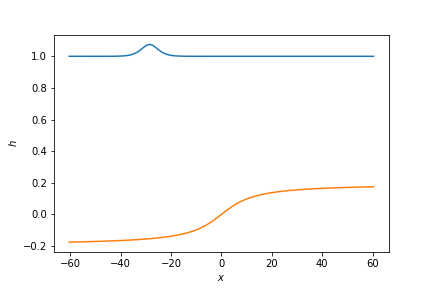
\includegraphics[scale=.6]{../../Simulations/DDM_NSWE_Serre/Figures/bottom.png}
	\captionof{figure}{Profiles of the bottom and the initial solution \label{fig:bottom}}
\endgroup 

\subsubsection{Interface boundary conditions}

\indent The interface boundary conditions applied in this problem are essentially the same as described above (equations \ref{eq:IBCNSWE} and \ref{eq:TBCSerre}), with only a small modification in the TBCs for the Serre subdomain : as the dispersive part of the Serre equations requires three boundary conditions, we consider two TBCs for its left boundary and one for the right, but constructed by the same principle (imposition of the solution of the advection step).

\indent Therefore, if we denote by the index $N$ the common point between $\Omega_1$ and $\Omega_2$, and by $2N$ the common point between $\Omega_2$ and $\Omega_3$, the interface boundary conditions four our coupling are : 

\begin{enumerate}
	\item Advection step : 
		\begin{equation*}
			\begin{gathered}
				u^{1,n}_{j,A} = u^{2,n-1}_{j}, \qquad j \in \{N+1,N+2,N+3\} \\
				u^{2,n}_{j,A} = u^{1,n-1}_{j}, \qquad j \in \{N-3,N-2,N-1\} \\
				u^{2,n}_{j,A} = u^{3,n-1}_{j}, \qquad j \in \{2N+1,2N+2,2N+3\} \\
				u^{3,n}_{j,A} = u^{2,n-1}_{j}, \qquad j \in \{2N-3,2N-2,2N-1\} \\ 
			\end{gathered}
		\end{equation*}
	\item Dispersive step :
		\begin{equation}
			\label{eq:TBCSerre}
			\begin{gathered}
				u^{2,n}_{j,D} = u^{2,n}_{j,A}, \qquad j=N,N+1 \\ 
				u^{2,n}_{2N,D} = u^{2,n}_{2N,A}
			\end{gathered}
		\end{equation}
\end{enumerate} 

\indent Concerning the external boundaries of $\Omega$, we always consider for the right boundary the standard "open boundary conditions" for the finite volume scheme, and we make tests with different conditions for the left boundary. We recall that open boundary conditions are imposed by simply reflecting the solution ($h$ and $u$) around the boundary to the ghost cells : 

\begin{equation}
	\label{eq:openBC}
	\begin{gathered}
		u^{3,n}_{3N+j,A} = u^{3,n-1}_{3N+1-j}, \qquad j \in \{1,2,3\}
	\end{gathered}
\end{equation}

\subsubsection{Test with open left boundary conditions}

\indent In this first test, we also impose to the left boundary the standard open boundary conditions, similarly to \eqref{eq:openBC}. We use as initial solution a solitary cnoidal wave with parameters $(a_0,a_1) = (1.0,0.075)$ and we perform the tests until the shock formation. As done previously, we compare the solution of the coupling with the solution provided by the NSWE applied to the entire domain. The solution in some instants is presented in the figure \ref{fig:ThreeSubdomains_open}, where the bottom was translated in order to appear in the plots.

\noindent

\begingroup
	\begin{minipage}{1.\linewidth}
		\includegraphics[scale=.6]{../../Simulations/DDM_NSWE_Serre/Figures/{ThreeSubdomains_open_A}.png}	
	\end{minipage}
	\begin{minipage}{1.\linewidth}
		\includegraphics[scale=.6]{../../Simulations/DDM_NSWE_Serre/Figures/{ThreeSubdomains_open_B}.png}	
	\end{minipage}
	\begin{minipage}{1.\linewidth}
		\includegraphics[scale=.6]{../../Simulations/DDM_NSWE_Serre/Figures/{ThreeSubdomains_open_C}.png}	
	\end{minipage}
	\begin{minipage}{1.\linewidth}
		\includegraphics[scale=.6]{../../Simulations/DDM_NSWE_Serre/Figures/{ThreeSubdomains_open_D}.png}	
	\end{minipage}
	\captionof{figure}{Result of the coupling and of the NSWE in the entire domain, for open boundary conditions on the left boundary. The bottom was translated to the appear in the plots \label{fig:ThreeSubdomains_open}}
\endgroup 

\subsubsection{Tests with a constant height imposed on the left boundary}

\indent ...
